\chapter{Introduction}
\label{Chapter:Intro}



%%%%%%%%%%%%%%%%%%%%%%%%%%%%%%%%%%%%%%%%%%%%%%%%%%%%%%%%%
%                                                       %
%                   S E C T I O N                       %
%                                                       %
%%%%%%%%%%%%%%%%%%%%%%%%%%%%%%%%%%%%%%%%%%%%%%%%%%%%%%%%%
\section{Software Crisis}  \label{Intro:Crisis}

Software ``production'' is inherently different from manufacturing production. Every software project is unique. Despite tremendous research effort invested by the software engineering community for the past several decades to build reliable software efficiently and effectively, software development methods, as currently practiced, still remain largely an art. Software development is slow, expensive and error prone, often resulting in products with large number of defects which cause serious problems in usability, reliability and performance.

According to \textit{the Chaos Report} \cite{Standish:1994} published by the Standish group, companies in the United States spent around \$250 billion on software development per year on approximately 175,000 projects. Only 16\% of these projects finished on schedule and within budget. 31\% were cancelled before completion mainly due to quality problems for losses of about \$81 billion. 53\% exceeded their original budgets by an average of 189\% for losses of about \$59 billion. Those projects that made it to completion delivered an average of 42\% of the planned features. The direct cost of these failures and overruns were just the tip of the iceberg. The loss of indirect opportunity costs were not measured in the report, but could easily be trillions of dollars.

A report \cite{Peterson:1997} from the Software Engineering Institute (SEI) indicated that out of 542 software organizations participating in a CMM maturity assessment, 67\% of them were at the lowest maturity level (level 1), and 20\% were at maturity level 2. The software process at level 1 was characterized as \textit{ad hoc} and sometimes \textit{chaotic}. Inputs to the process were ill-defined, and the transition from inputs to final products was uncontrolled. The development process was so reactive that management control was impossible. The development process at level 2 was better, because earlier successes on projects with similar applications could be repeated. However, there was still no visibility into how software products were produced, and any pertubation to development teams or development resources could easily cause project failure. Combined, 87\% of the software organizations surveyed were unable to control their development processes, nor were they unable to consistently develop software products on schedule and within budget. 

Uncontrollable and non-repeatable processes cause many problems to software development organizations. For example, it becomes hard to ensure software quality, hard to make reliable effort and schedule estimation, and impossible to allocate resources efficiently.



%%%%%%%%%%%%%%%%%%%%%%%%%%%%%%%%%%%%%%%%%%%%%%%%%%%%%%%%%
%                                                       %
%                   S E C T I O N                       %
%                                                       %
%%%%%%%%%%%%%%%%%%%%%%%%%%%%%%%%%%%%%%%%%%%%%%%%%%%%%%%%%
\section{Software Measurement, Process Improvement and Predictions}  \label{Intro:Measurement}

It is conventional wisdom that \textit{you can neither predict nor control what you cannot measure} \cite{DeMarco:1982}. Consistent measurement is a key component in establishing a scientific basis for software engineering. Software metrics are capable of quantifying software products and their development processes in an objective way. They make certain aspects of processes and products more visible, and give us better understanding of relationships between development activities and the attributes of software products they affect. As a result, various measurement programs have been developed to improve software organizations' development processes and their capability to produce software products in a controllable and repeatable manner. 

Effective measurement programs help software organizations understand their capabilities, so that they can develop achievable plans for producing and delivering software products. Furthermore, continual measurement can provide an effective foundation for managing process improvement activities. The end result is that software organizations can have controllable and repeatable development processes, and thus the ability to make reliable predictions about their development activities.

Indeed, software measurement is always at the core of software process improvement and assessment programs, such as PSP \cite{Humphrey:1995, Humphrey:1996}, CMM \cite{Humphrey:1989, Paulk:1993, Humphrey:1995}, ISO 9001 \cite{ISO9001:1987}, SPICE \cite{ISO:1998, Eman:1998} and BOOTSTRAP \cite{Kuvaja:1994}. Industrial experience \cite{Grady:1987} has demonstrated that so long as measurement programs are conscientiously followed, they can help software organizations achieve improved development processes, both in the short run and in the long run. Controllable and repeatable processes are essential for software organizations to make reliable predictions about their development activities, such as those in SLIM \cite{Putnam:1978, SLIM} and COCOMO \cite{Cocomo:1981, Cocomo:2000}, so that they can make realistic and achievable plans.

%Mature software development process bring benefits to software development organizations, such as on-time within-budget delivery of high quality software products, improved predictability and productivity. Software measurements play an ever important role as a software organization's development process matures.



%%%%%%%%%%%%%%%%%%%%%%%%%%%%%%%%%%%%%%%%%%%%%%%%%%%%%%%%%
%                                                       %
%                   S E C T I O N                       %
%                                                       %
%%%%%%%%%%%%%%%%%%%%%%%%%%%%%%%%%%%%%%%%%%%%%%%%%%%%%%%%%
\section{Problem Statement}  \label{Intro:Problem}


Despite the potential of software measurement in theory and positive experiences in reality, effective application appears far from mainstream in practice. For example, a recent case study \cite{Kulik:2003} surveyed 630 software professionals. Only 27\% of the ``best practice'' organizations responded that reliance on metrics and measurements when making project-related decisions was \textit{very} or \textit{extremely} important, while just 2\% of ``all other'' organizations responded the same way. 

Several reasons can be hypothesized.

All measurement activities compete for resources. An important question for a software organization committing itself to measurement program is whether the benefit from improved development processes outweighs the cost. Existing measurement programs tend to be very expensive. For example, the PSP uses manual metrics collection. Every time a compilation error occurs, the developer has to stop his/her current work, and record details about the error. It is not only tedious, but also susceptible to bias, error, omission, and delay. CMM requires that in all key process areas measurements be taken to determine the status of the activities. A study by Herbsleb, et al. \cite{Herbsleb:1997} found that it took on average 2 years per level for a software development organization to get from CMM level 1 to level 3, and that the cost ranged from \$500 to \$2000 per employee per year. Quantitative measurement is explicitly addressed in CMM level 4, and Humphrey himself admitted that ``the greatest potential problem with the managed process (i.e. level 4) was the cost of gathering data, and that there were an enormous number of potentially valuable measures of the software process, but such data were expensive to gather and to maintain'' \cite{Humphrey:1988}. Due to high cost associated with metrics collection and analysis, it is a daunting task to apply measurement best practices to improve an software organization's development process in practice. 

%Realizing the difficulties, agile community has been promoting ``softer'' metrics for project management for years\cite{Beck:2000}.

%CMM Level 5 requires (1) the support of automatic gathering of process data, and (2) the use of process data both to analyze and to modify the process to prevent problems and to improve efficiency.

%All process maturity and assessment frameworks include measurement as means to help software organizations to improve their development process (for example, CMM prescribes ). However, none of them deals with software metrics collection and analysis explicitly. 

%The GQM paradigm does provide a top-down approach to software measurement based on high level business goals, and metrics are used to deliver the necessary information to make decisions in order to improve software development process. However, it's an abstract model and the actual metrics collection and analysis are not a part of the paradigm.

%Software organizations are left on their own to determine how the software measurement processes should be implemented.
	

Even if we successfully overcome the issues with metrics collection, there is still difficulty of using software measures for the purpose of project management and process improvement. Traditional approaches use ``historical project database'' as a baseline for comparison with metrics from the current project, which tend to yield results not easily translated into practice. They typically involve the following basic procedure: (1) collect a set of process and product metrics, such as size, effort, complexity, and defects, for a set of completed software projects, (2) generate a model to fit the observed data, (3) and claim that the model can be used to predict characteristics of future projects. Project management and process improvement is based on the predictions made by the models. For example, a model might predict that a future project of size \textit{S} would require \textit{E} person-months of effort; another model might predict that a future implementation of a module with complexity \textit{C} would be prone to defects with density \textit{D}. 

This model-based process prediction technique is used in many forms, such as in the PSP and COCOMO. It faces a number of limitations. First, the predictive power of these models depends crucially on how well model calibration is performed. In order to use the model off-the-shelf, practitioners must confirm that the set of projects used to calibrate the model are ``comparable'' to the project they wish to predict. Otherwise, the model must be recalibrated using the data in the organization's historical project database, to avoid the problem of comparing apples to oranges. This involves replicating the model-building method within the practitioner's organization, with the risk that the applications, personnel, and resources may have already changed, and the context of future projects may differ from those in the historical project database. Second, model-based process prediction assumes the process of a software organization is predictable. However, according to the SEI survey \cite{Peterson:1997} mentioned in Section \ref{Intro:Crisis}, 67\% of the surveyed organizations were at the lowest CMM maturity level. By definition, the software processes at that level are \textit{ad hoc} and sometimes \textit{chaotic}, and they change as work changes. As a result, it is generally impossible to make predictions for these organizations. Lastly, and most fundamentally, the majority of the models that are available are built to compare a set of finished projects. This may be useful in initial project planning, but we are more interested in managing a project and guiding it to successful completion. How do we compare metrics from completed projects to the one that is still in progress?

%\textcolor{red}{TO INCOPORATE: A traditional approach to use of project metrics for management begins by collecting ``final'' values of these measures over a set of completed projects. This ``historical project metrics repository'' is then used as a baseline for comparison with data from a current project. While this can be a useful approach to initial project planning, it has a number of obvious limitations. First, the historical projects must be ``comparable'' to the current one, which can be hard when applications, personnel, and resources are changing. Second, and more fundamentally, how do you usefully compare data from a completed project to one that is still in progress? The automated nature of metrics collection and analysis in Hackystat allows a different use of these metrics. Instead of trying to compare data from already completed projects to the current in-progress project, we can instead compare snapshots of data collected from a single Project over various points in time to each other. For example, if Active Time was consistently 30 hours per day from the start of a Project until recently, but has now dropped to 15 hours per day, then management may need to consider obtaining additional resources for this Project, or else adjust the scope. As another example, if coverage used to be almost 100\% but has been gradually dropping over time, then management may need to re-allocate resources to improve quality assurance.}


The result is the dilemma we are facing today. Almost all software organizations are aware of the benefits of a mature development process and the value of measurement programs in achieving it. However, few of them are capable of implementing a successful measurement program in practice. The difficulties lie in (1) the overhead and the cost associated with metrics collection and analysis, and (2) the difficulty in translating metrics research results into practice.






%%%%%%%%%%%%%%%%%%%%%%%%%%%%%%%%%%%%%%%%%%%%%%%%%%%%%%%%%
%                                                       %
%                   S E C T I O N                       %
%                                                       %
%%%%%%%%%%%%%%%%%%%%%%%%%%%%%%%%%%%%%%%%%%%%%%%%%%%%%%%%%
\section{Proposed Solution - Software Project Telemetry}  \label{Intro:Solution}

To address the problem, I propose a novel, light-weight measurement approach called \textit{software project telemetry}. It includes both (1) highly automated measurement machinery for metrics collection and analysis, and (2) a methodology for in-process, empirically-guided software development process problem detection and diagnosis. 

In this approach, sensors collect software metrics automatically and unobtrusively. Metrics are abstracted in real time to telemetry streams, charts, and reports, which represent high-level perspectives on software development. Telemetry trends are the basis for decision-making in project management and process improvement. Unlike traditional approaches which are primarily based on historical project databases and focused on comparison of similar projects, software project telemetry emphasizes project dynamics and in-process control. It combines both the precision of traditional project management techniques and the flexibility promoted by agile community.






\subsection{Measurement Machinery in Software Project Telemetry}
\label{Intro:Solution:MeasurementMachinery}

In software project telemetry, sensors collect metrics \textit{automatically}. Sensors are software tools that monitor some form of state in project development environment \textit{unobtrusively}. Some examples are (1) a sensor for an IDE monitoring developer activities, such as code editing effort, compilation attempts and results, etc., or (2) a sensor for a version control system monitoring code check-in and check-out activities, and computing \textit{diff} information between different revisions. There can be many possibilities. However, the key is that sensors are designed to collect metrics \textit{automatically} and \textit{unobtrusively} in order to keep metrics collection overhead sufficiently low, so that developers are not distracted from their primary task -- developing software products instead of recording process and product metrics.

The metrics collected by sensors are time-stamped, and the time stamp is always significant in metrics analysis. \textit{Telemetry streams}, \textit{charts}, and \textit{reports} capture high-level perspectives on software development, while \textit{the telemetry language} facilitates interactive exploration of these perspectives. Figure \ref{fig:TelemetryReportChartStream} shows the relationship between telemetry streams, charts, and reports. 

\begin{figure}[p]
  \centering
  \includegraphics[height=0.90\textheight]{figures/TelemetryReportChartStream}
  \caption{The Relationship between Telemetry Streams, Charts, and Reports} 
  \label{fig:TelemetryReportChartStream}
\end{figure}





\subsubsection{Telemetry Reports}

A telemetry report is a named set of telemetry charts that can be generated for a specified project over a specified time interval. The goal of a telemetry report is to discover how the trajectory of different process and product metrics might influence each other over time, and whether these influences change depending upon context.

For example, Figure \ref{fig:TelemetryReportChartStream} shows a telemetry report consisting of two charts. Both charts show \textit{Unit Test Dynamics Telemetry}, which is an analysis of trends in the percentage of active time\footnote{Active time is a proxy for developer effort writing and editing code inside an IDE.} allocated to testing, the percentage of source code devoted to testing, and the percentage of test coverage that results from this effort and code. The charts share the same time interval and project. The only difference is that they show unit test dynamics data for two different modules in the same project. Interestingly, the unit test dynamics telemetry trends for the two modules have a very different shape, indicating differences in the underlying approach to development of these two modules.



\subsubsection{Telemetry Charts}

A telemetry chart is a named set of telemetry streams that can be generated for a specified project over a specified time interval. The goal of a telemetry chart is to display the trajectory over time of one or more process or product metrics.

For example, Figure \ref{fig:TelemetryReportChartStream} shows two instances of the same telemetry chart. The chart, entitled \textit{Unit Test Dynamics Telemetry}, contains three telemetry streams: \textit{ActiveTime-Percentage}, \textit{JavaSLOC-Percentage}, and \textit{JavaCoverage-Percentage}. You can see references to these three streams in the legend accompanying each chart. The legends also illustrate that telemetry streams can be parameterized: the top chart contains streams parameterized for the \textit{hackyZorro} module, while the bottom chart contains streams parameterized for the \textit{hackyCGQM} module.




\subsubsection{Telemetry Streams}

Telemetry streams are sequences of a single type of process or product data for a single project over a specified time interval. Telemetry streams are best thought of as a kind of abstract data type representing one or more series of metric data values of a similar type. In addition, they support basic arithmetic operations.

For example, Figure \ref{fig:TelemetryReportChartStream} shows three kinds of telemetry streams, each with its own color. The red line in each chart is an \textit{ActiveTime-Percentage} stream, the blue line in each chart is a \textit{JavaSLOC-Percentage} stream, and the green line in each chart is a \textit{JavaCoverage-Percentage} stream. 

The time interval covered by telemetry stream is divided into periods. The data points in each telemetry stream reflect the state of some key aspect of the software system under study during each period. The period can be relatively fine-grained such as daily, or more coarse-grained such as weekly or monthly. Two types of information are typically represented by the data points: 

\begin{itemize}
	\item Aggregation information - The metrics metrics values can be accumulated over the time period. Some examples are total coding effort, total lines added or deleted in the source code, total number of new bugs reported, etc.
	
	\item Snapshot information - The metrics are only meaningful at a specific point in time. Some examples are the size of the source code, the number of open bugs, etc. Usually, the snapshot is taken at the beginning or at the end of the period.
\end{itemize}


%\begin{figure}[tbp]
%  \centering
%  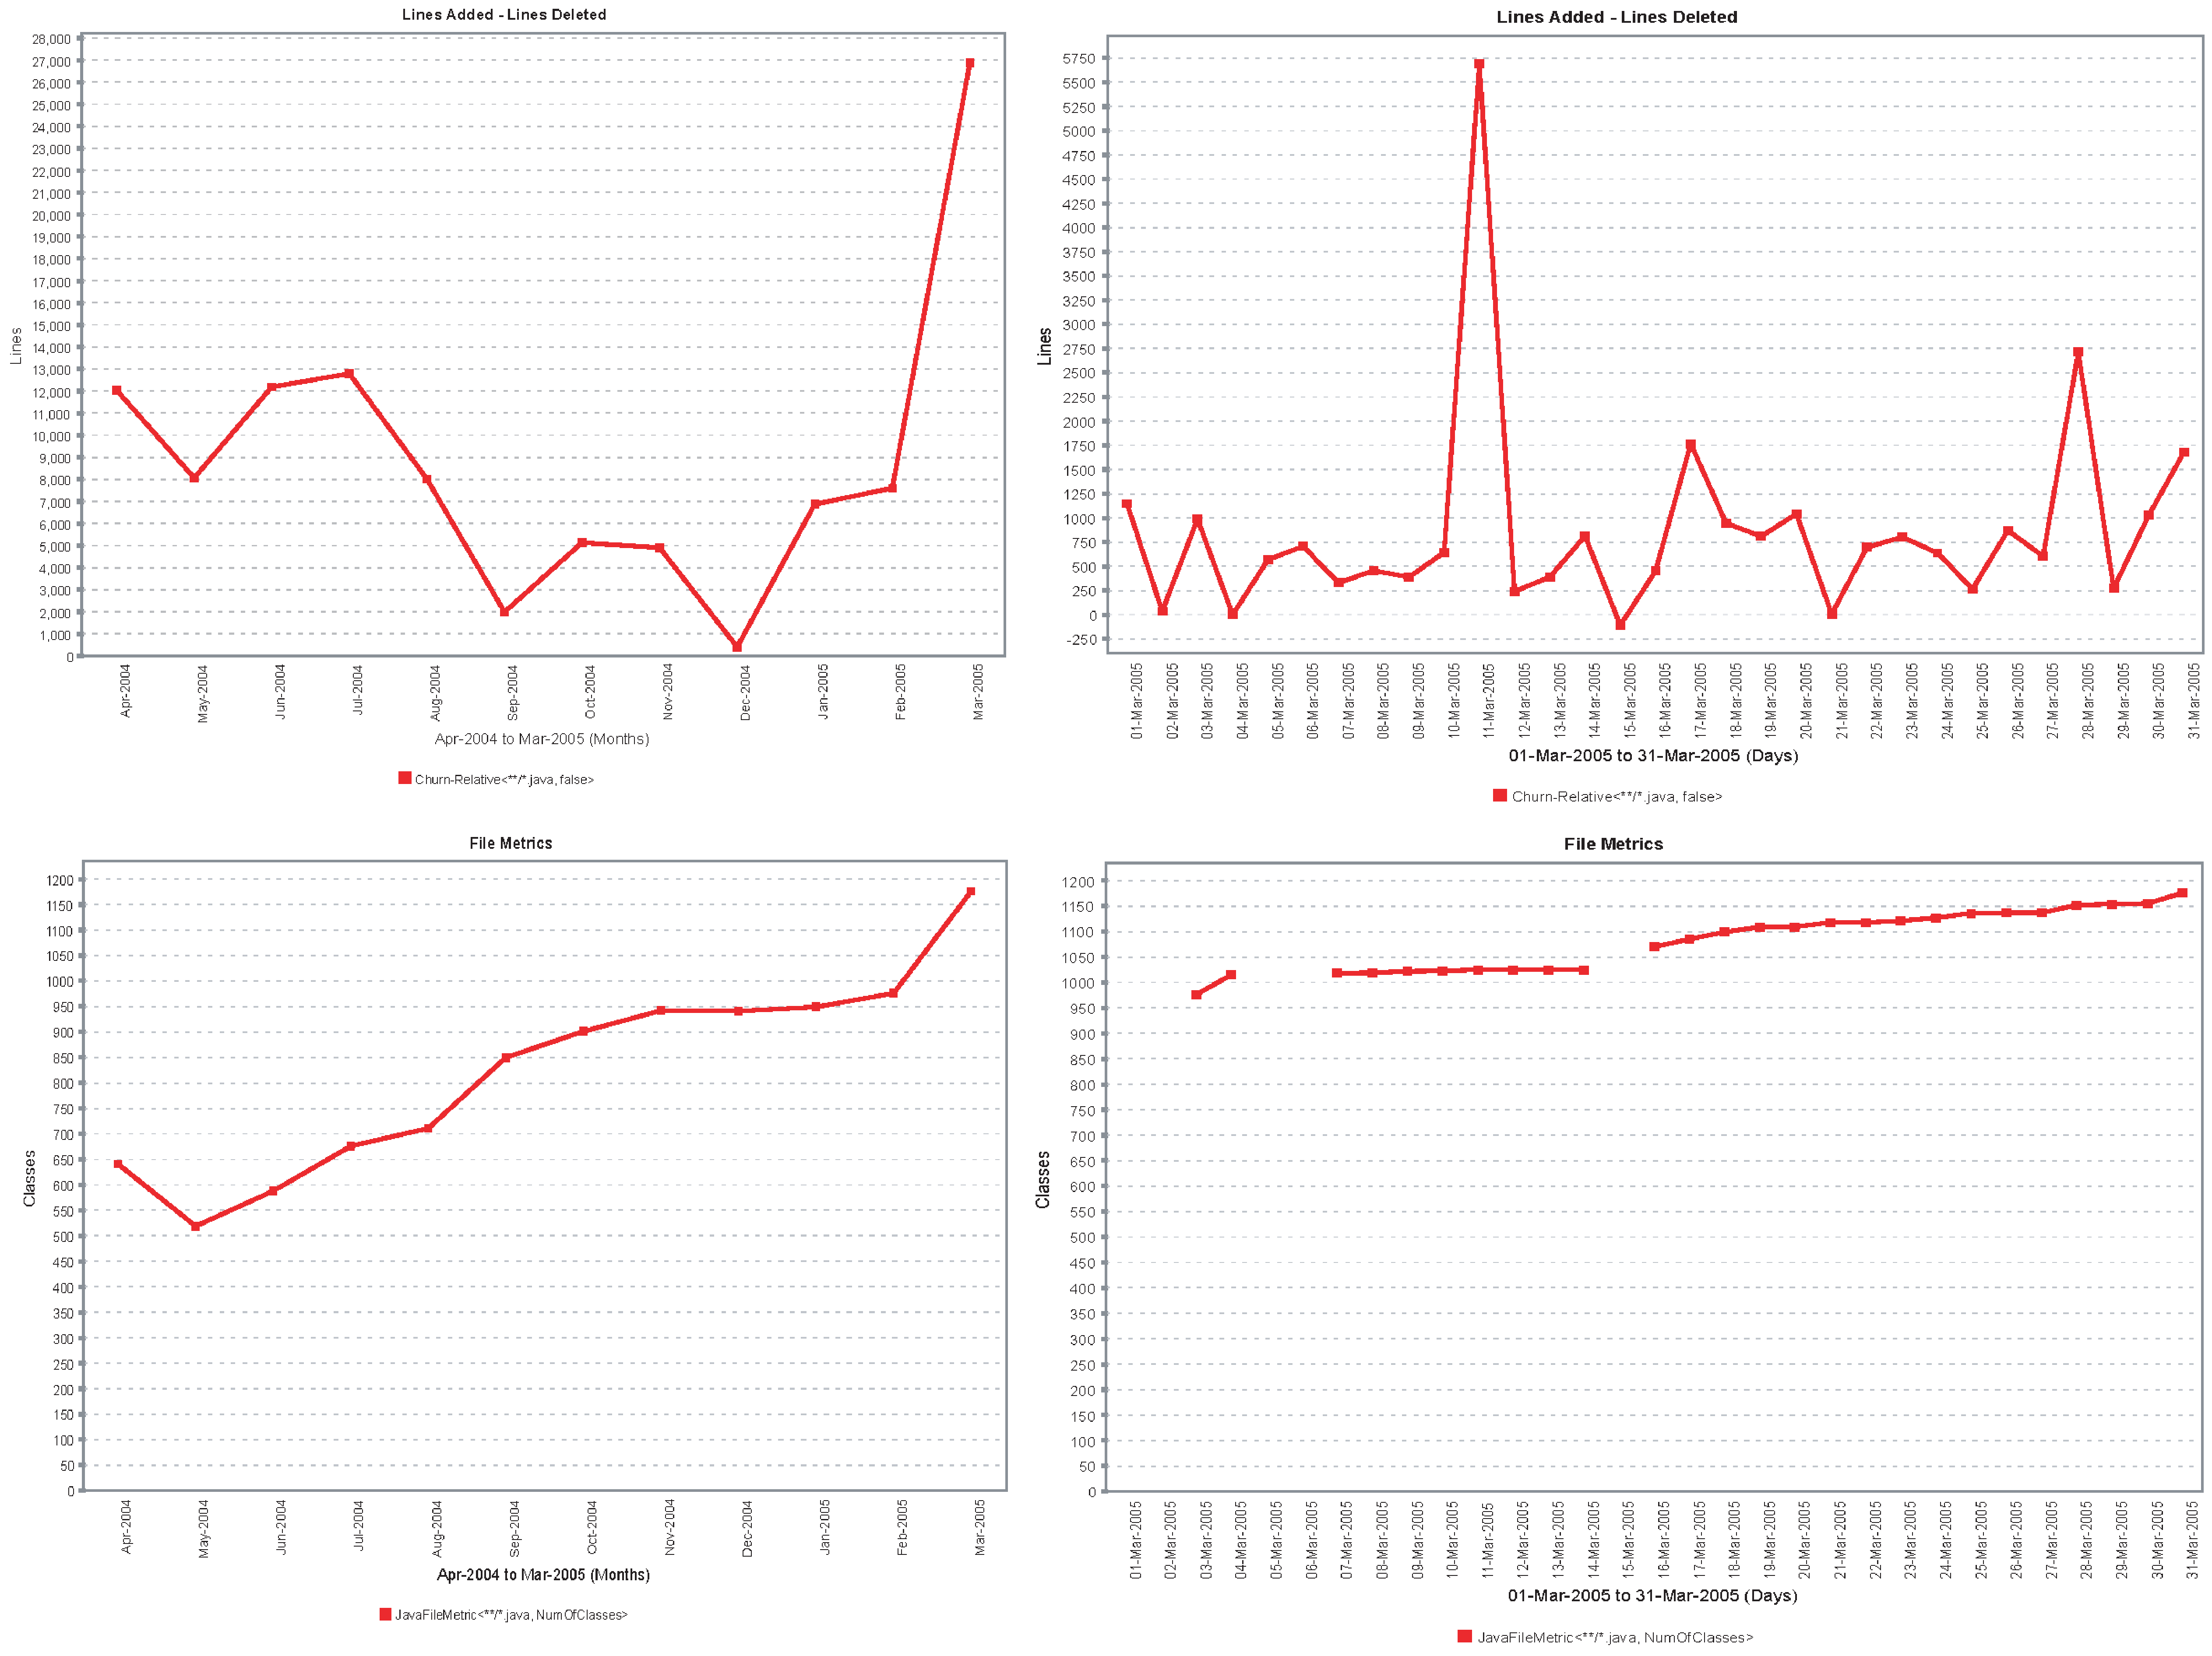
\includegraphics[width=1.00\textwidth]{figures/TelemetryStreamIntro}
%  \caption{Telemetry Streams} 
%  \label{fig:TelemetryStreamIntro}
%\end{figure}

\begin{figure}[p]
  \centering
  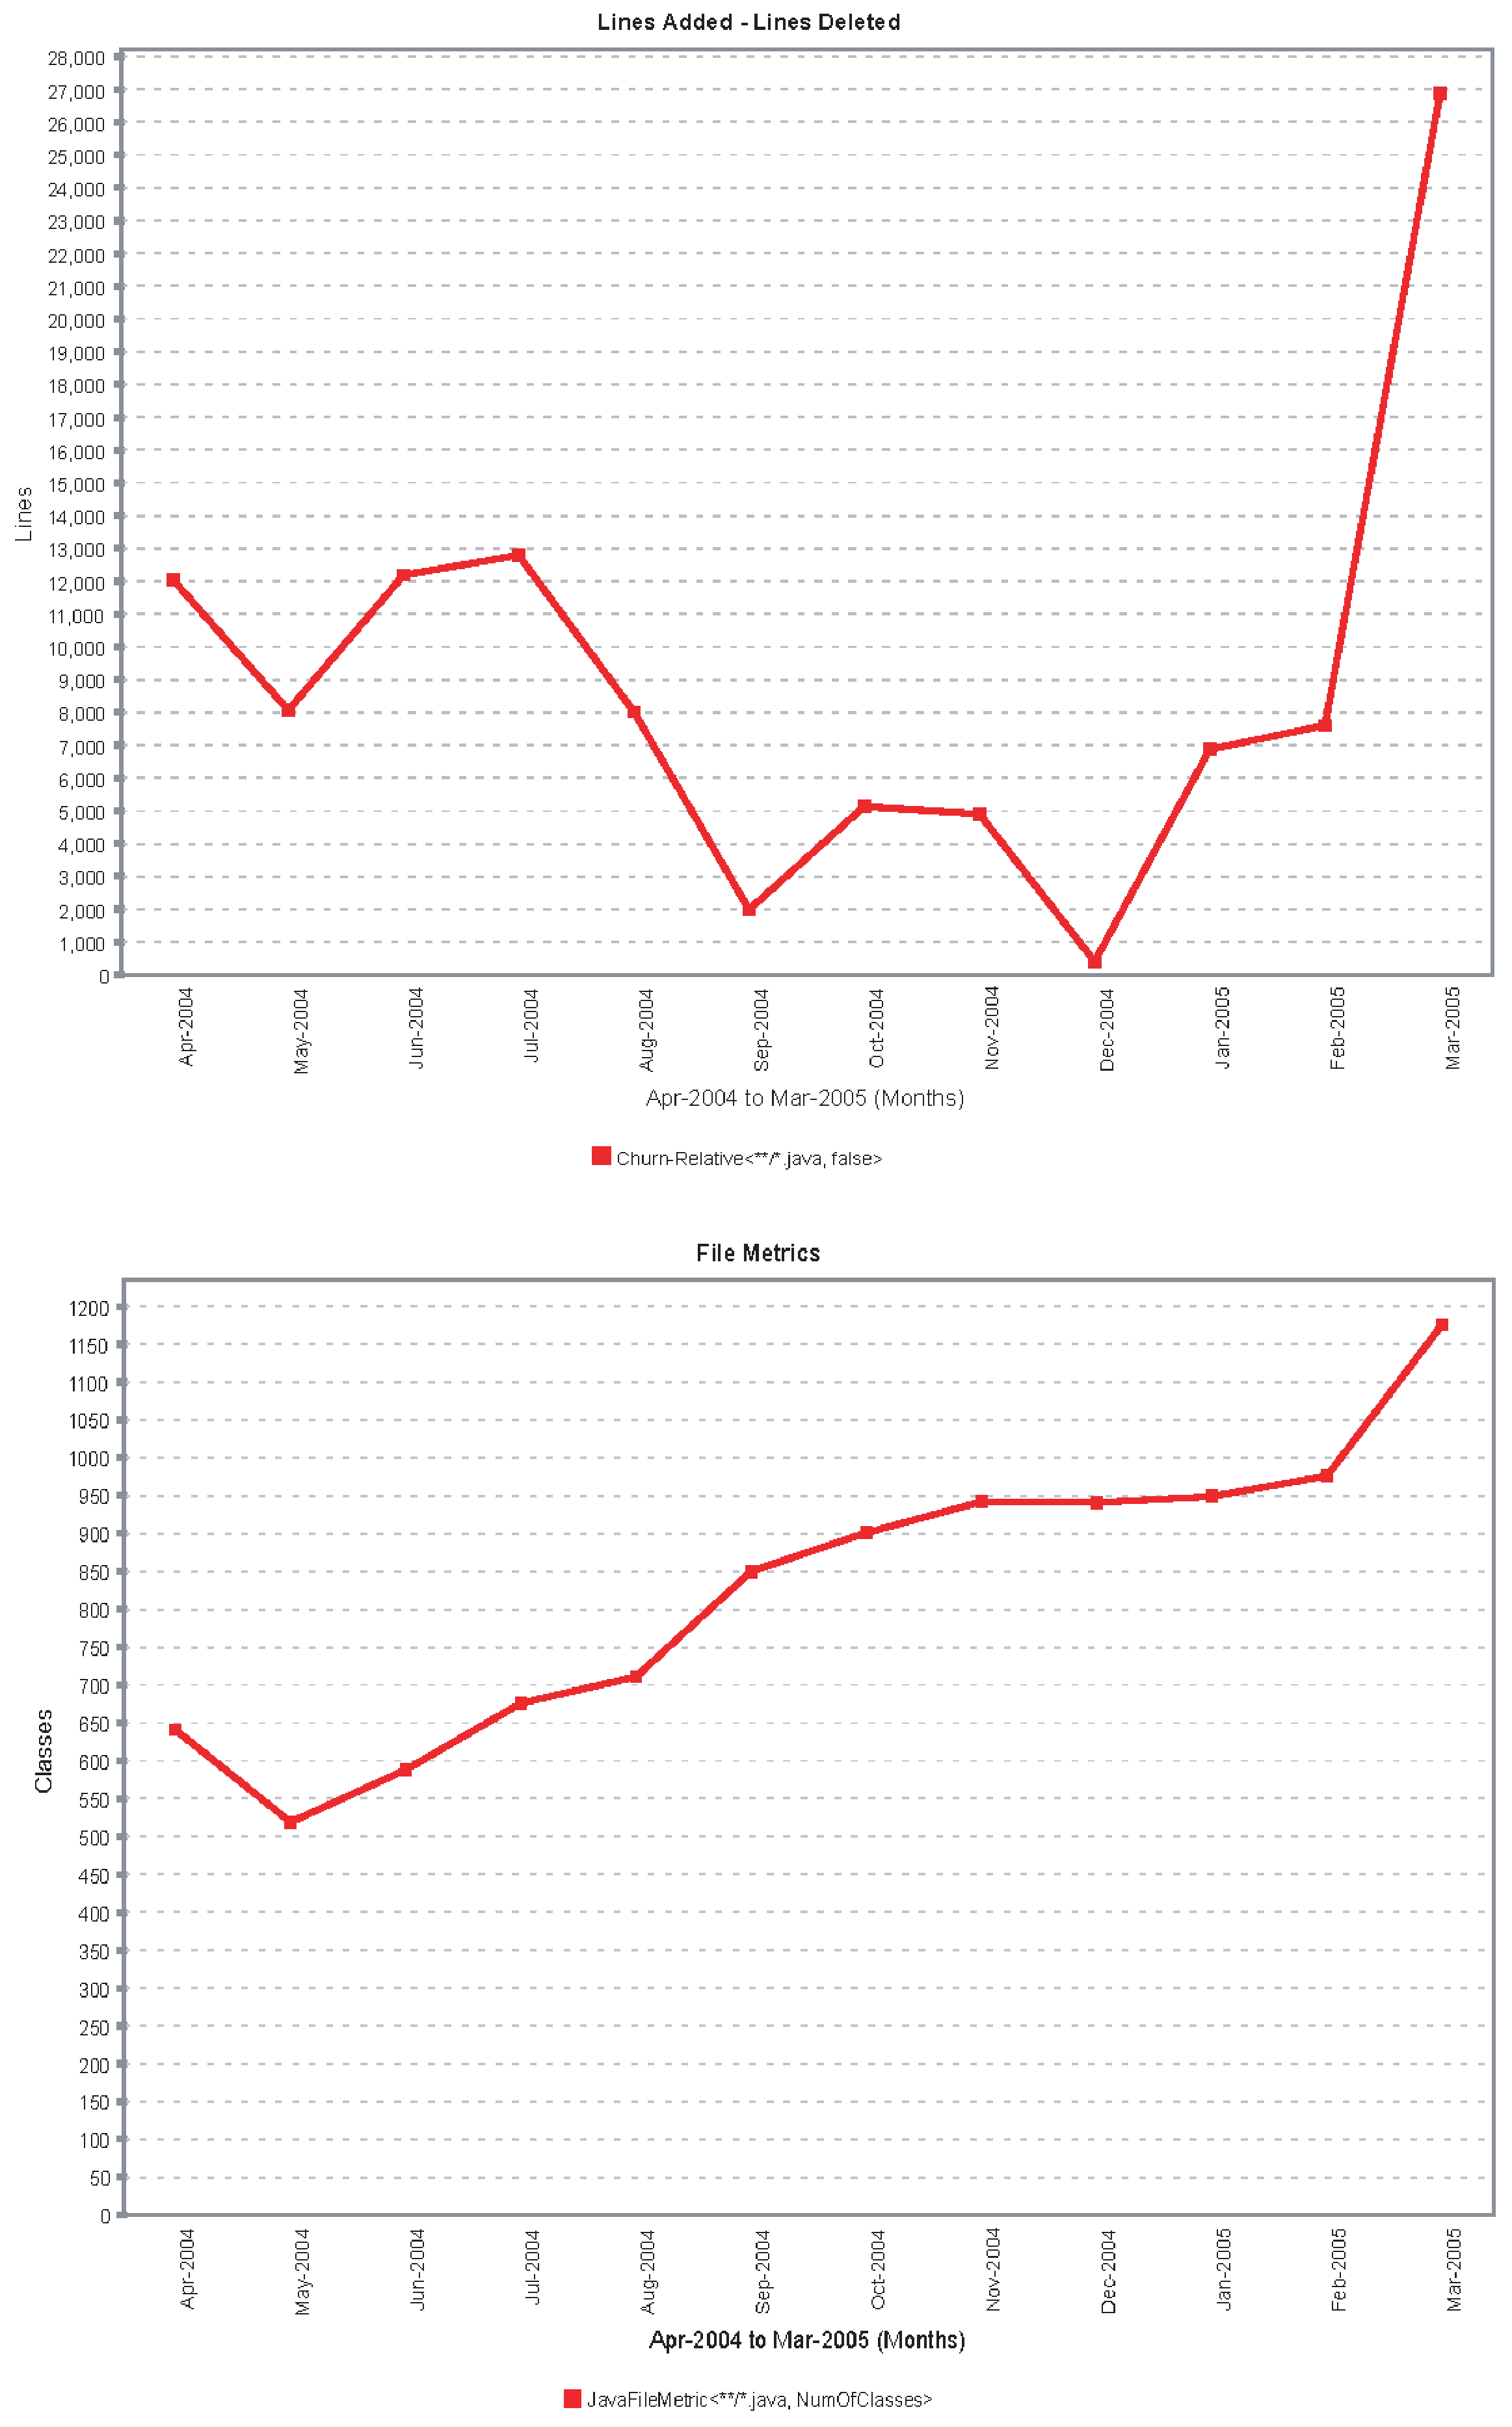
\includegraphics[height=0.90\textheight]{figures/TelemetryStreamIntro-Monthly}
  \caption{Telemetry Streams (Monthly)} 
  \label{fig:TelemetryStreamIntroMonthly}
\end{figure}

\begin{figure}[p]
  \centering
  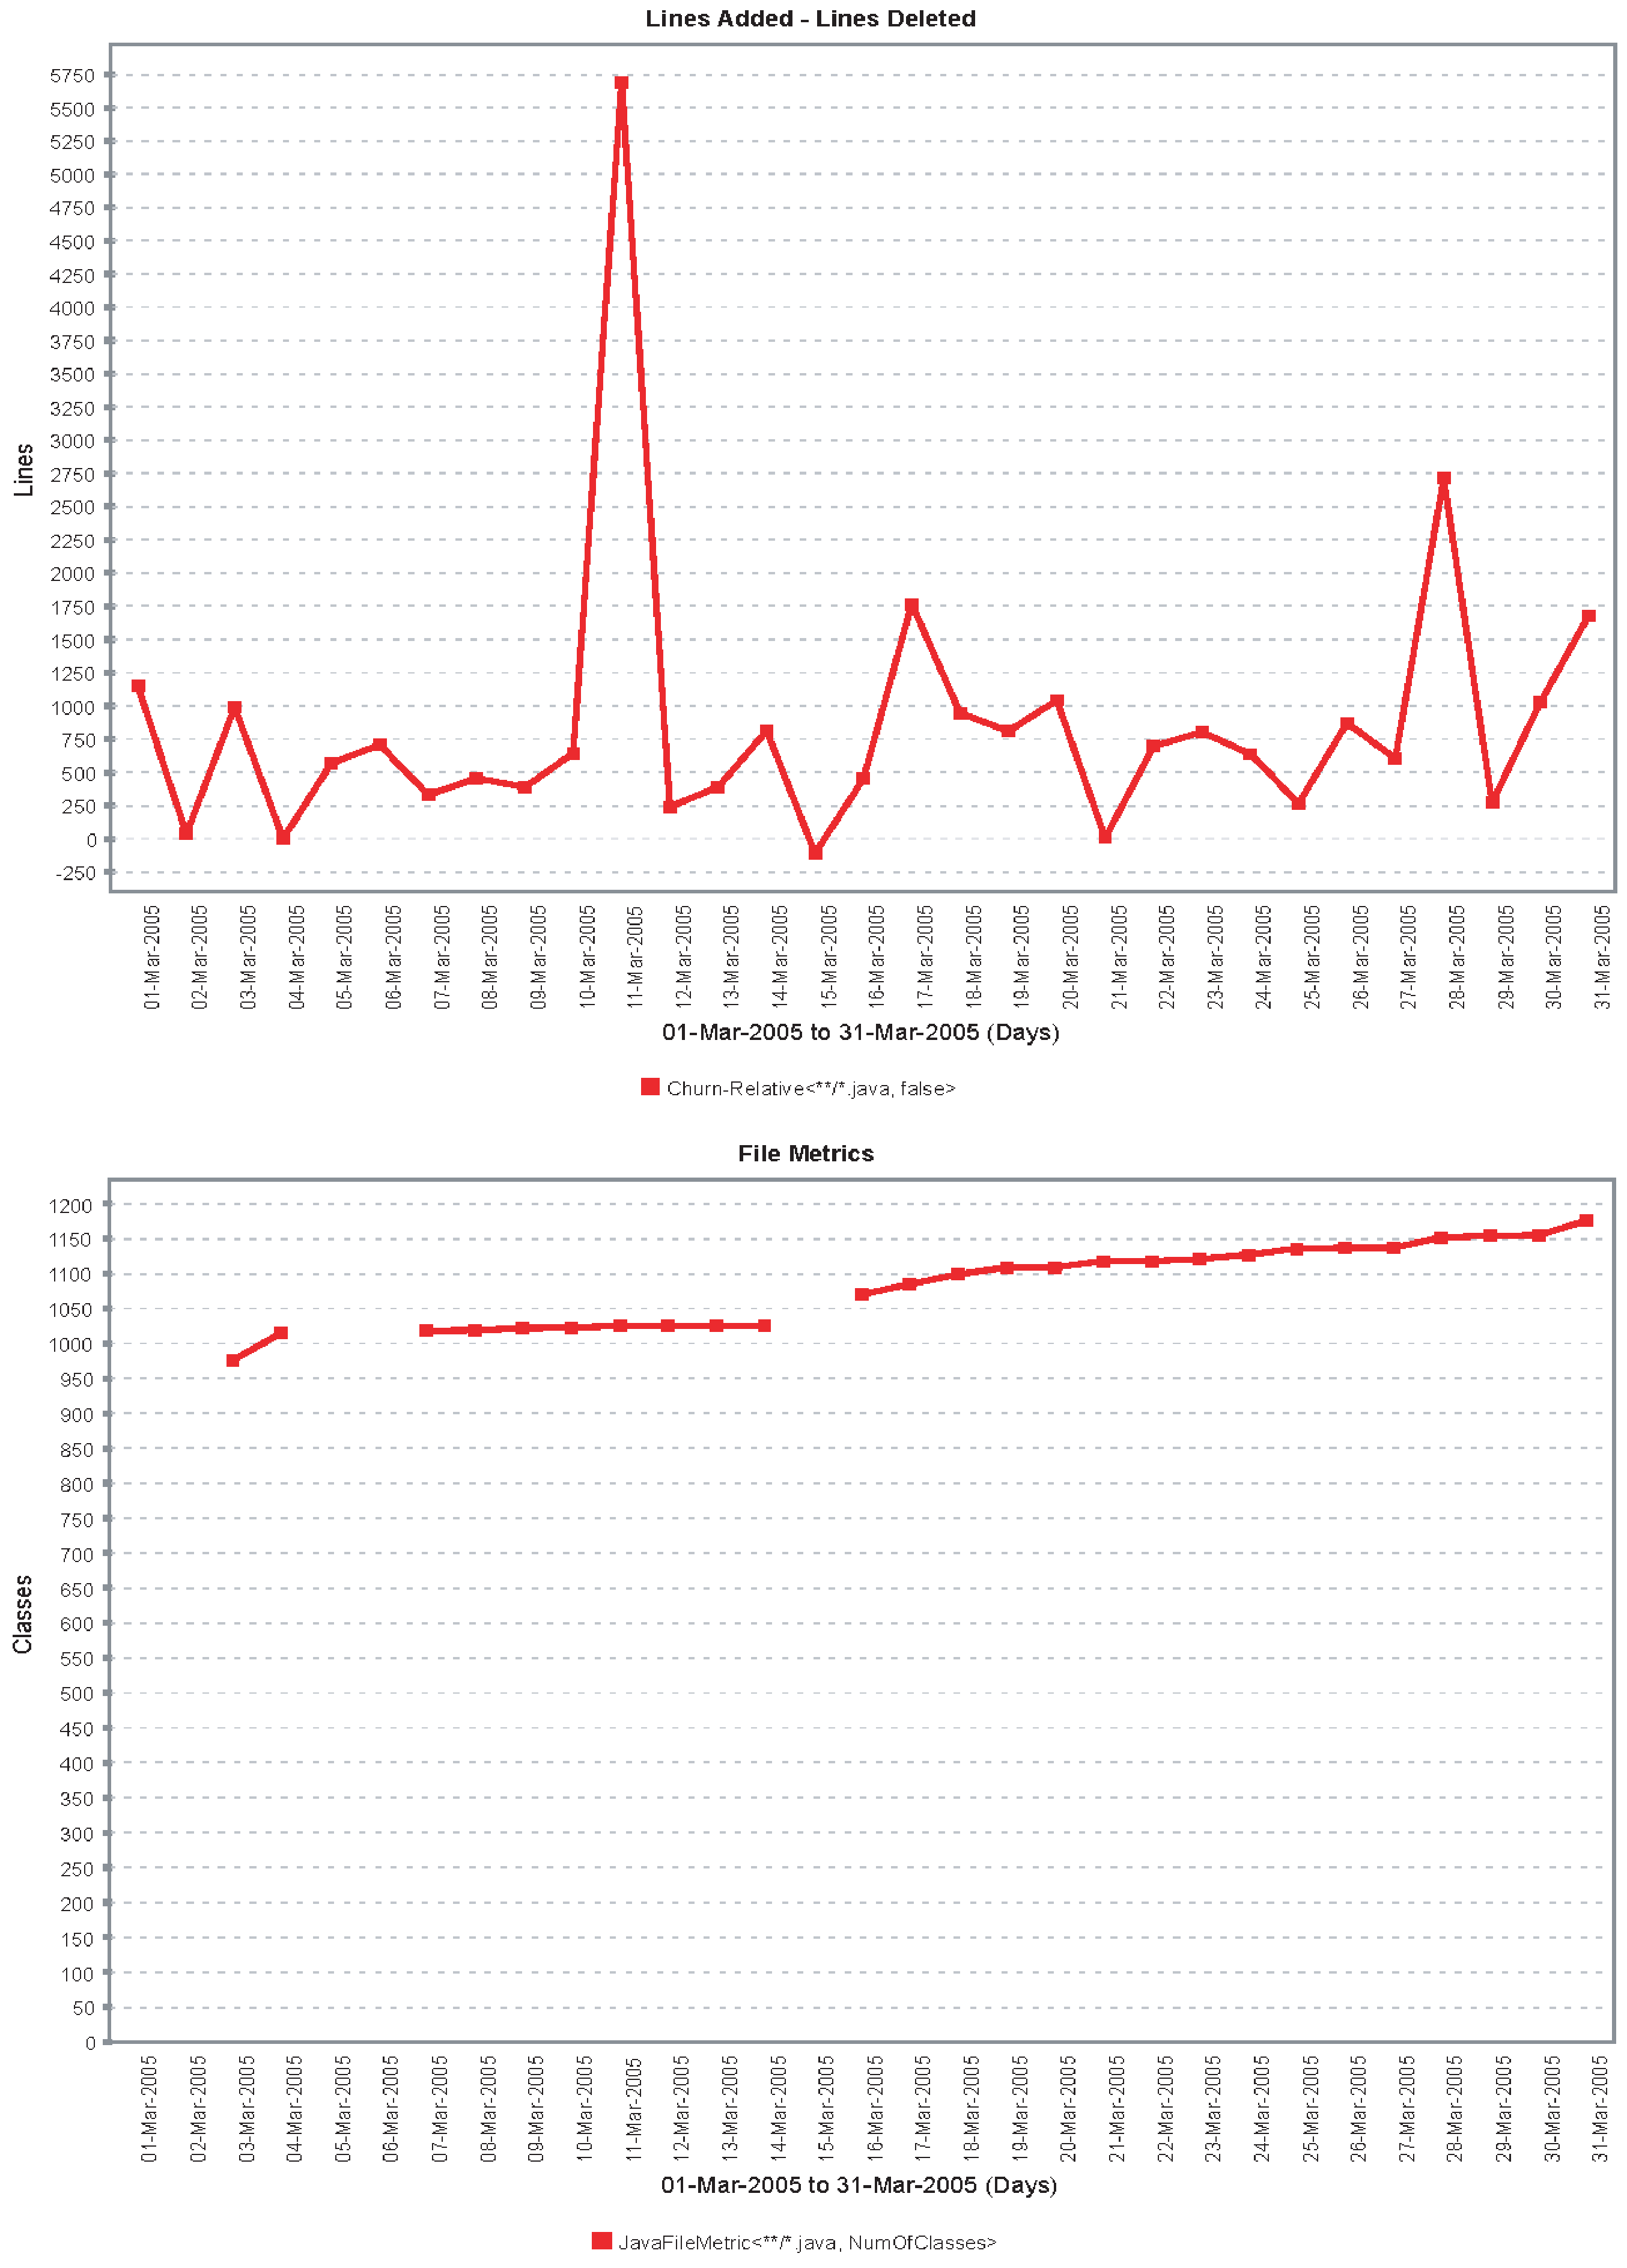
\includegraphics[height=0.90\textheight]{figures/TelemetryStreamIntro-Daily}
  \caption{Telemetry Streams (Daily)} 
  \label{fig:TelemetryStreamIntroDaily}
\end{figure}

Figure \ref{fig:TelemetryStreamIntroMonthly} and \ref{fig:TelemetryStreamIntroDaily} show four telemetry streams. 
The data points in the upper telemetry streams in the two figures represent aggregation information. In this case, they are the net increase in the number of lines in the source code. The time period in Figure \ref{fig:TelemetryStreamIntroMonthly} is month, and each data point represents code size increase for the entire month. The time period in Figure \ref{fig:TelemetryStreamIntroDaily} is day, and each data point represents code size increase for one single day. 
The data points in the lower telemetry streams in the two figures represent snapshot information. In this case, they are the number of Java classes in a software system. Though the two streams use monthly and daily period respectively, the data points actually represent the snapshot of the system size at the end of each period.

The advantage of using telemetry streams is that they show the entire history of the status of some state in project development environment, and thus help project manager detect changes in the development process. Telemetry streams may contain missing data, such as in the case of the lower one in Figure \ref{fig:TelemetryStreamIntroDaily}. While complete data provide the best support for project management, occasional drop of data point should have little impact on their value for decision-making. As a result, analyses built on top of telemetry streams can exhibit graceful degradation, providing value even when only partial data is available.


%\begin{figure}[tbp]
%  \centering
%  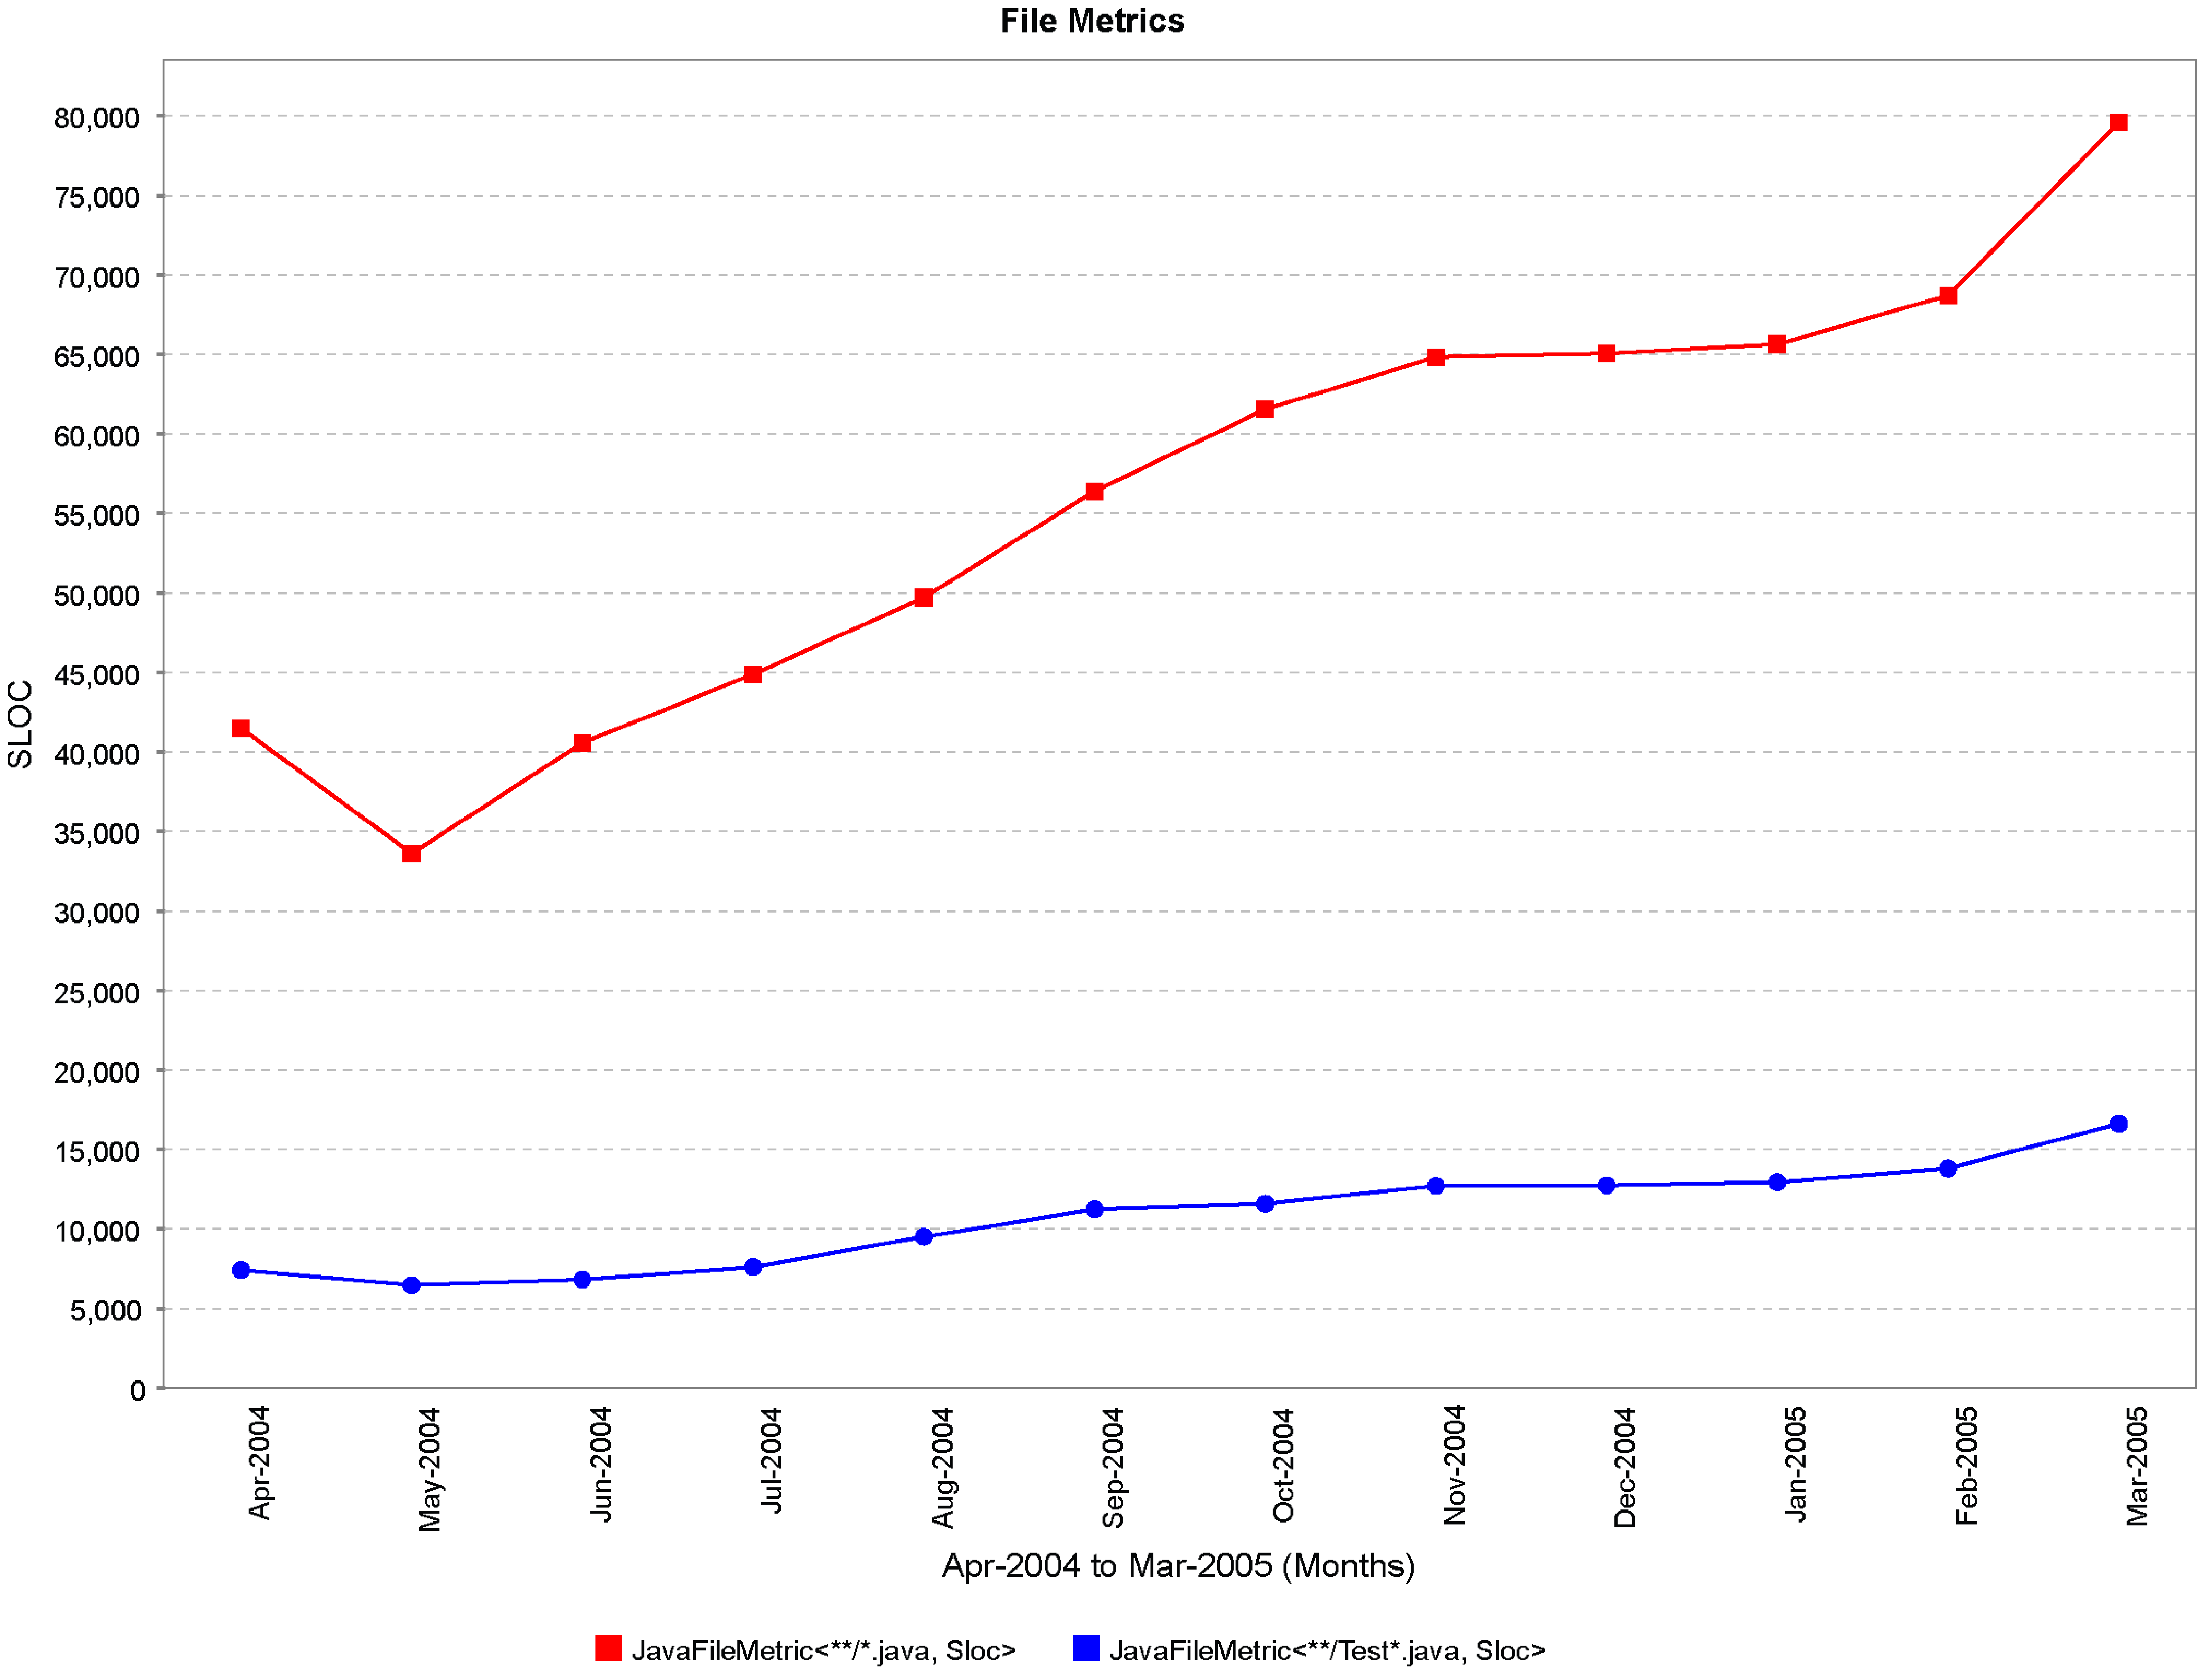
\includegraphics[width=1.00\textwidth]{figures/TelemetryChartIntro}
%  \caption{Telemetry Chart} 
%  \label{fig:TelemetryChartIntro}
%\end{figure}
%
%\textit{Telemetry chart} is visual representation of telemetry streams. It consists of one or more telemetry streams sharing common horizontal and vertical axises. The horizontal axis is always time intervals (daily, weekly, monthly, etc.). The information represented by vertical axis varies depending on the telemetry streams displayed in the chart. It can be programming effort (hours), system size (LOC), or anything else. For example, Figure \ref{fig:TelemetryChartIntro} is a telemetry chart containing two telemetry streams -- source lines of code (SLOC) for an entire software system, and test code in the system, respectively. 
%
%\begin{figure}[p]
%  \centering
%  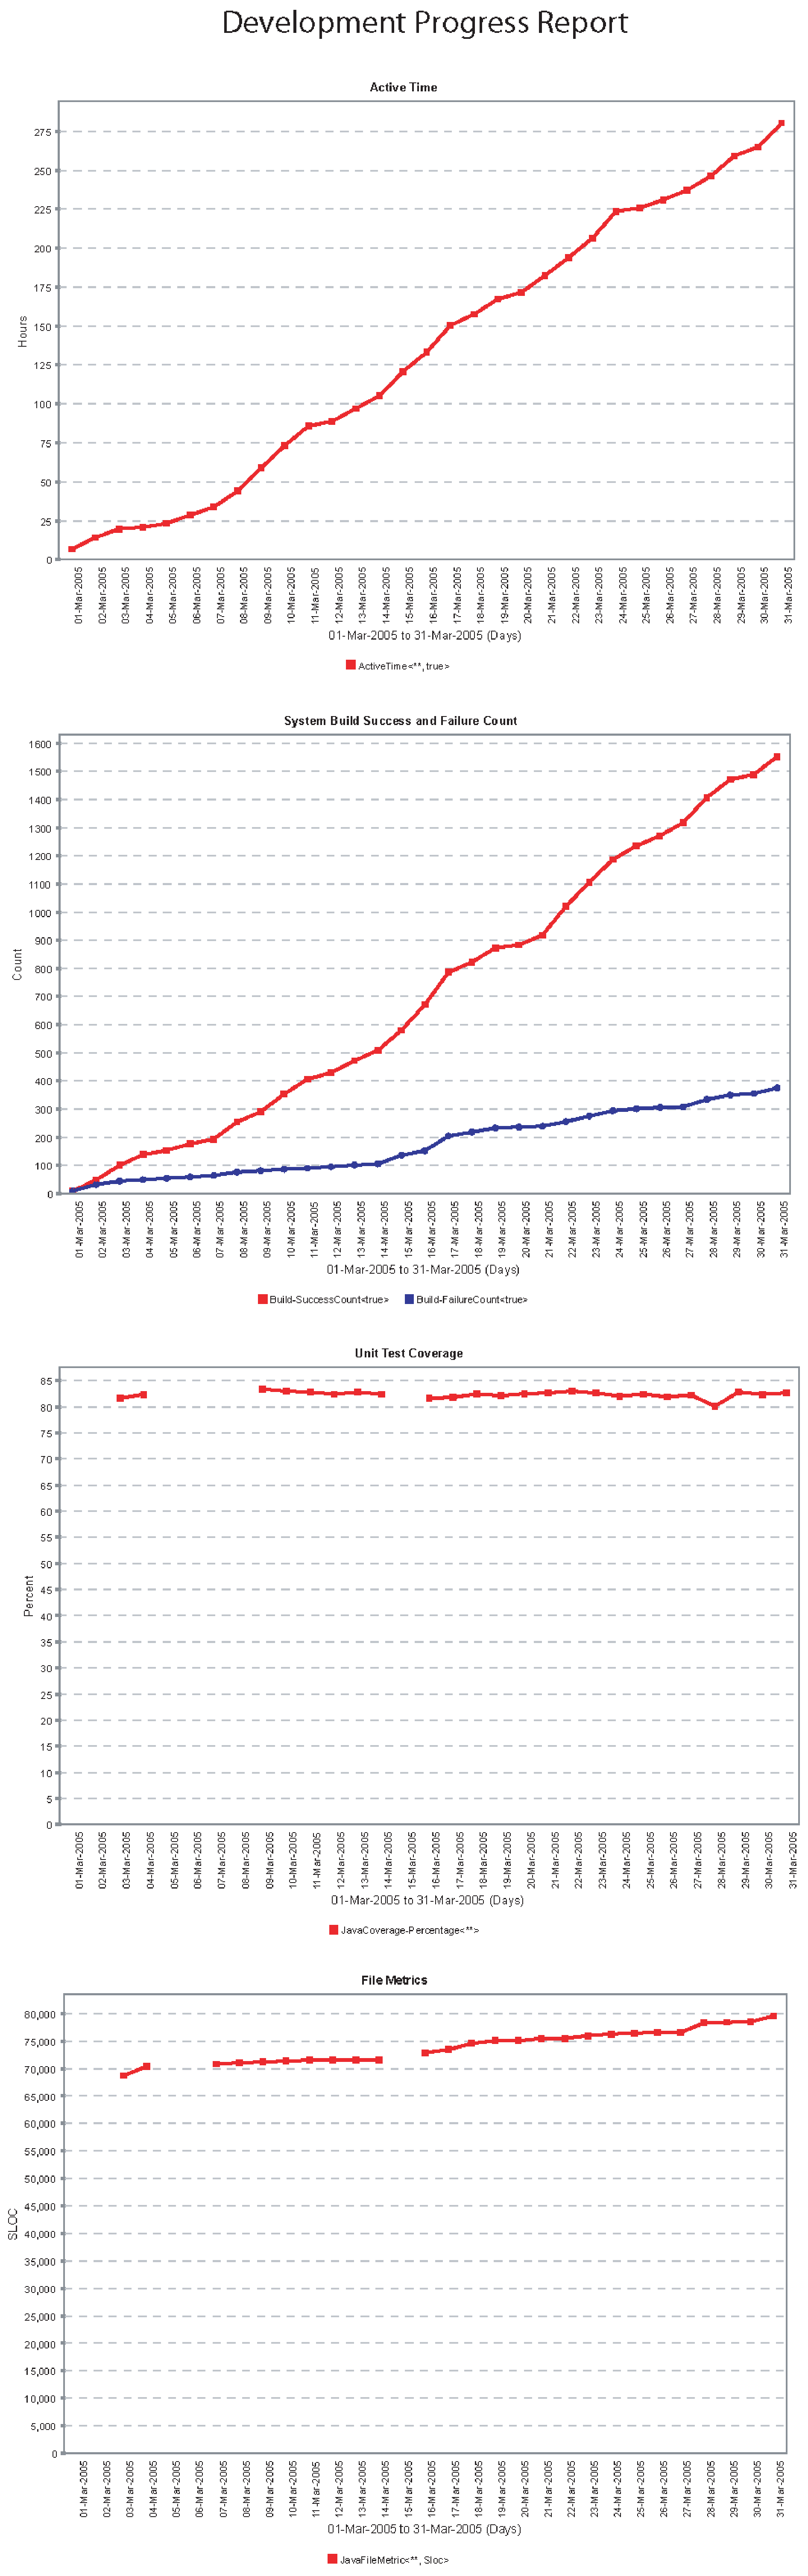
\includegraphics[height=0.90\textheight]{figures/TelemetryReportIntro}
%  \caption{Telemetry Report} 
%  \label{fig:TelemetryReportIntro}
%\end{figure}
%
%\textit{Telemetry report} groups different telemetry charts with the same horizontal axis (i.e. representing the same intervals). The charts can have different vertical axises. For example, Figure \ref{fig:TelemetryReportIntro} is a telemetry report for an overview of the development progress of a software project for the month of May 2005 on a daily basis. The report contains 4 charts on effort, size, test, and build.
%
%The idea behind both telemetry chart and report is that by juxtaposing different telemetry streams for the same period, it makes it easier for a project manager to detect how different telemetry streams co-varies, which is important to software project telemetry process methodology (Section \ref{Intro:Solution:ProcessMethodology}).


\subsubsection{Telemetry Language}


\textit{Telemetry language} provides a flexible mechanism to construct telemetry streams, charts, and reports, and facilitates interactive exploration of different perspectives on software development. The language has the following simple syntax, and the details can be found in Section \ref{Telemetry:Language}.

\begin{verbatim}
  streams <StreamName> (<ParameterList>) = {
    <DocumentationString>, <UnitLabel>, 
    <ReductionFunctionExpresion>
  };
    
  chart  <ChartName>  (<ParameterList>) = {
    <ChartTitile>, <StreamExpression>
  };
    
  report <ReportName> (<ParameterLilst>) = {
    <ReportTitle>, <ChartExpression>
  };
\end{verbatim}










\subsection{Process Methodology in Software Project Telemetry}
\label{Intro:Solution:ProcessMethodology}

Telemetry streams contain software process and product metrics, and they are the basis of project management and process improvement. Telemetry charts and reports provide visualizations for project managers that help monitor software development status, and that can detect undesirable process changes. By juxtaposing different telemetry streams for the same time period, a project manager can detect co-variances between them. For example, one might find that a drop in test coverage is always associated with an increase in the number of open bugs. Depending on what interval scale is used, one may even find that a decrease in test coverage is always followed by an increase in open bugs\footnote{The observation of timing sequence of events is not always guaranteed. Fine-grained intervals may introduce noise, while coarse-grained intervals may lose information. This is one of the reasons why telemetry analyses offer different interval scales, such as daily, weekly, and monthly.}. This kind of information is important to software project management, because it suggests a plausible causal relationship -- low test coverage causes more bugs to slip through to the production stage. Based on this information, the project manager can implement changes to increase test coverage, and continue to use telemetry streams to monitor whether it indeed results in a decrease of the number of open bugs. At the same time, the project manager can monitor other telemetry streams, and check whether this corrective action has any unintended side effect to the development process. For example, he/she may wish to monitor productivity related telemetry streams to make sure that there is no reduction in developer productivity. 

In general, telemetry-based software project management involves cycles of:

\begin{enumerate}
  \item \textit{Problem Detection} --- Use telemetry streams to monitor the development of a software project. Detect anomalies and undesirable trends in telemetry streams.
    
  \item \textit{Process Improvement Hypothesis Generation} --- Determine possible causes for the problem, and possible measures to correct it.
  
  \item \textit{Process Change Implementation} --- Implement corrective measures.
  
  \item \textit{Hypothesis Validation and Impact Analysis} --- Determine whether the problem goes away after corrective measures are implemented, and whether there are any unintended side effects caused by the corrective measures.

\end{enumerate}

The cycle continues until the project reaches completion.

%Software process improvement hypothesis can be embedded in the design of telemetry streams, and by monitoring the change of those streams, a software manager can either confirm or reject the process improvement hypothesis.
















%%%%%%%%%%%%%%%%%%%%%%%%%%%%%%%%%%%%%%%%%%%%%%%%%%%%%%%%%
%                                                       %
%                   S E C T I O N                       %
%                                                       %
%%%%%%%%%%%%%%%%%%%%%%%%%%%%%%%%%%%%%%%%%%%%%%%%%%%%%%%%%
\section{Thesis Statement}  \label{Intro:Thesis}

The main claim of this thesis is that software project telemetry provides an effective automated approach to in-process, empirically-guided software development process problem detection and diagnosis. 

Compared to traditional model-base process prediction approaches, management with software project telemetry has many advantages. 

Software project telemetry is easier to use and cheaper to implement. It does not require software organizations to accumulate process and product metrics of finished projects in a historical database. Nor does it require expensive and error-prone model calibration before it can be used to make predictions. Instead, it focuses on evolutionary processes in development, and relies on metrics from an earlier stage of product development of the same project to make short-term predictions. For example, if system test coverage used to be almost 100\% but has been gradually dropping over time, then it may be a signal for management to re-allocate resources to improve project quality assurance. As a result, software project telemetry is best suited for in-process monitoring and control.

Software project telemetry is robust. The information contained in telemetry streams is seldom affected when there is occasional metrics drop out, and analyses still provide decision-making value even if metrics collection starts midway through a project. 

Software project telemetry is flexible. There are no required set of metrics to be collected. Different software organizations can collect different set of metrics according to their objectives, cost-benefit trade-offs, and measurement capabilities. For example, organizations with low process visibility can start with simple metrics such as source code size, and more metrics can be collected as their process matures and visibility increases.

%Software project telemetry can be used stand-alone as a light-weight method for project management. It can also supplement existing approaches such as GQM paradigm and maturity based process improvement frameworks, as the following example illustrates:
%
%\begin{itemize}
%	\item GQM paradigm can be used to generate high level goals and guide what telemetry streams to monitor. These telemetry streams, in turn, determine what software metrics need to be collected by sensors.
%	\item Process maturity determines the visibility of development activities. It is used to determine what software metrics we can collect and interpret in a meaningful way. With maturer processes, more metrics can be collected.
%	\item Software project telemetry provides an effective automated framework for metrics collection, analysis, and in-process, empirically-guided software process improvement hypothesis generation and validation. 
%\end{itemize}

%Together, they provide not only a meaningful context but also a practical approach to software measurement. 










%%%%%%%%%%%%%%%%%%%%%%%%%%%%%%%%%%%%%%%%%%%%%%%%%%%%%%%%%
%                                                       %
%                   S E C T I O N                       %
%                                                       %
%%%%%%%%%%%%%%%%%%%%%%%%%%%%%%%%%%%%%%%%%%%%%%%%%%%%%%%%%
\section{Evaluation}  \label{Intro:Evaluation}

My dissertation claim will be evaluated through three case studies:

\begin{itemize}
	\item A case study with student users in software engineering classes to gather their opinions about software project telemetry. \textbf{[completed]}
	\item A case study in CSDL using software project telemetry to investigate and improve the build process of a large-scale software development project.
	\item A case study at Ikayzo with open-source project developers to gather their opinions about software project telemetry.
\end{itemize}

%The case studies \textcolor{red}{will} adopt mixed methods research paradigm collecting and analyzing both qualitative and quantitative data with priority given to qualitative information.

%To a larger extent software engineering is about how people interact with each other and interact with tools to product software products. Software project telemetry is no exception. It is a metrics-based approach to project management and process improvement. It is designed to automate tedious metrics collection tasks and provide metrics analysis support through high level telemetry perspectives of the development process. It is not designed to replace human judgment in project decision-making. An important goal of the evaluation is to understand how software project telemetry provides metrics collection and analysis support and how project manager and developers interact with the technology to make decisions. As a result naturalistic approach and qualitative data analysis are consistent with the overall goal of this evaluation (i.e. exploration of a phenomenon). %survey and ethnography

%Quantitative information such as the actual invocation of software project telemetry analysis will be used to assist or cross-validate the interpretation of qualitative findings when appropriate. The use of multiple forms of data collection and analysis have the potential to offset the weaknesses inherent within one method with the strengths of the other method.



%%%%%%%%%%%%%%%%%%%%%%%%%%%%%%%%%%%%%%%%%%%%%%%%%%%%%%%%%
%                                                       %
%                   S E C T I O N                       %
%                                                       %
%%%%%%%%%%%%%%%%%%%%%%%%%%%%%%%%%%%%%%%%%%%%%%%%%%%%%%%%%
%\section{Results}  \label{Intro:Results}






%%%%%%%%%%%%%%%%%%%%%%%%%%%%%%%%%%%%%%%%%%%%%%%%%%%%%%%%%
%                                                       %
%                   S E C T I O N                       %
%                                                       %
%%%%%%%%%%%%%%%%%%%%%%%%%%%%%%%%%%%%%%%%%%%%%%%%%%%%%%%%%
\section{Anticipated Contributions}  \label{Intro:Contribution}


The anticipated contributions of this research will be:

\begin{itemize}
	\item The concept of software project telemetry as an effective automated approach to in-process, empirically-guided software development process problem detection and diagnosis. 
  
  \item An implementation of software project telemetry which allows continuous monitoring of software project status, as well as generating and validating software process improvement hypothesis.
  
  \item The insights gained from the case studies regarding how to use software project telemetry effectively for project management and process improvement, as well as the adoption barrier of the technology.

\end{itemize}








%%%%%%%%%%%%%%%%%%%%%%%%%%%%%%%%%%%%%%%%%%%%%%%%%%%%%%%%%
%                                                       %
%                   S E C T I O N                       %
%                                                       %
%%%%%%%%%%%%%%%%%%%%%%%%%%%%%%%%%%%%%%%%%%%%%%%%%%%%%%%%%
\section{Dissertation Proposal Organization}  \label{Intro:Organization}

This dissertation \textcolor{red}{proposal} is organized into the following chapters:

\begin{itemize}
  \item {Chapter \ref{Chapter:Intro}} is this chapter where the problem statement and proposed solution is described.
  
  \item {Chapter \ref{Chapter:Telemetry}} describes software project telemetry in detail and how it facilitates software project management and process improvement.

  \item {Chapter \ref{Chapter:RelatedWork}} relates the current research to the broader context of existing work.
        
  \item {Chapter \ref{Chapter:Implementation}} details the design and implementation of software project telemetry.

  \item {Chapter \ref{Chapter:EvaluationStrategy}} gives a brief review of research methods and discusses the evaluation strategies of software project telemetry.
  
  \item {Chapter \ref{Chapter:EvaluationInClassroom}} \textcolor{red}{reports on a completed pilot} case study with student users in software engineering classes in which their opinions about software project telemetry were gathered.
  
  \item {Chapter \ref{Chapter:EvaluationInCSDL}} \textcolor{red}{outlines a planned} case study in CSDL using software project telemetry to investigate and improve the build process of a large-scale software development project.
 
  \item {Chapter \ref{Chapter:EvaluationInIkayzo}} \textcolor{red}{outlines a planned} case study at Ikayzo with open-source project developers gathering their opinions about software project telemetry.
 
  \item {Chapter \ref{Chapter:Conclusion}} concludes this dissertation
        \textcolor{red}{proposal with a discussion of the anticipated contributions and future directions}.
\end{itemize}


